\documentclass[tikz,border=0pt]{standalone}
\usepackage[T1]{fontenc}
\usepackage{helvet}
\renewcommand{\familydefault}{\sfdefault}
\usepackage{tikz}
\usetikzlibrary{arrows.meta,calc}

\definecolor{ink}{HTML}{14202B}
\definecolor{teal}{HTML}{0C5F59}
\definecolor{tealdeep}{HTML}{094E49}
\definecolor{paper}{HTML}{F4F1EA}
\definecolor{sand}{HTML}{E7E1D6}
\definecolor{agentgreen}{HTML}{14633A}
\definecolor{data}{HTML}{5C4A3A}
\definecolor{muted}{HTML}{526170}
\definecolor{line}{HTML}{D5D0C6}

\begin{document}
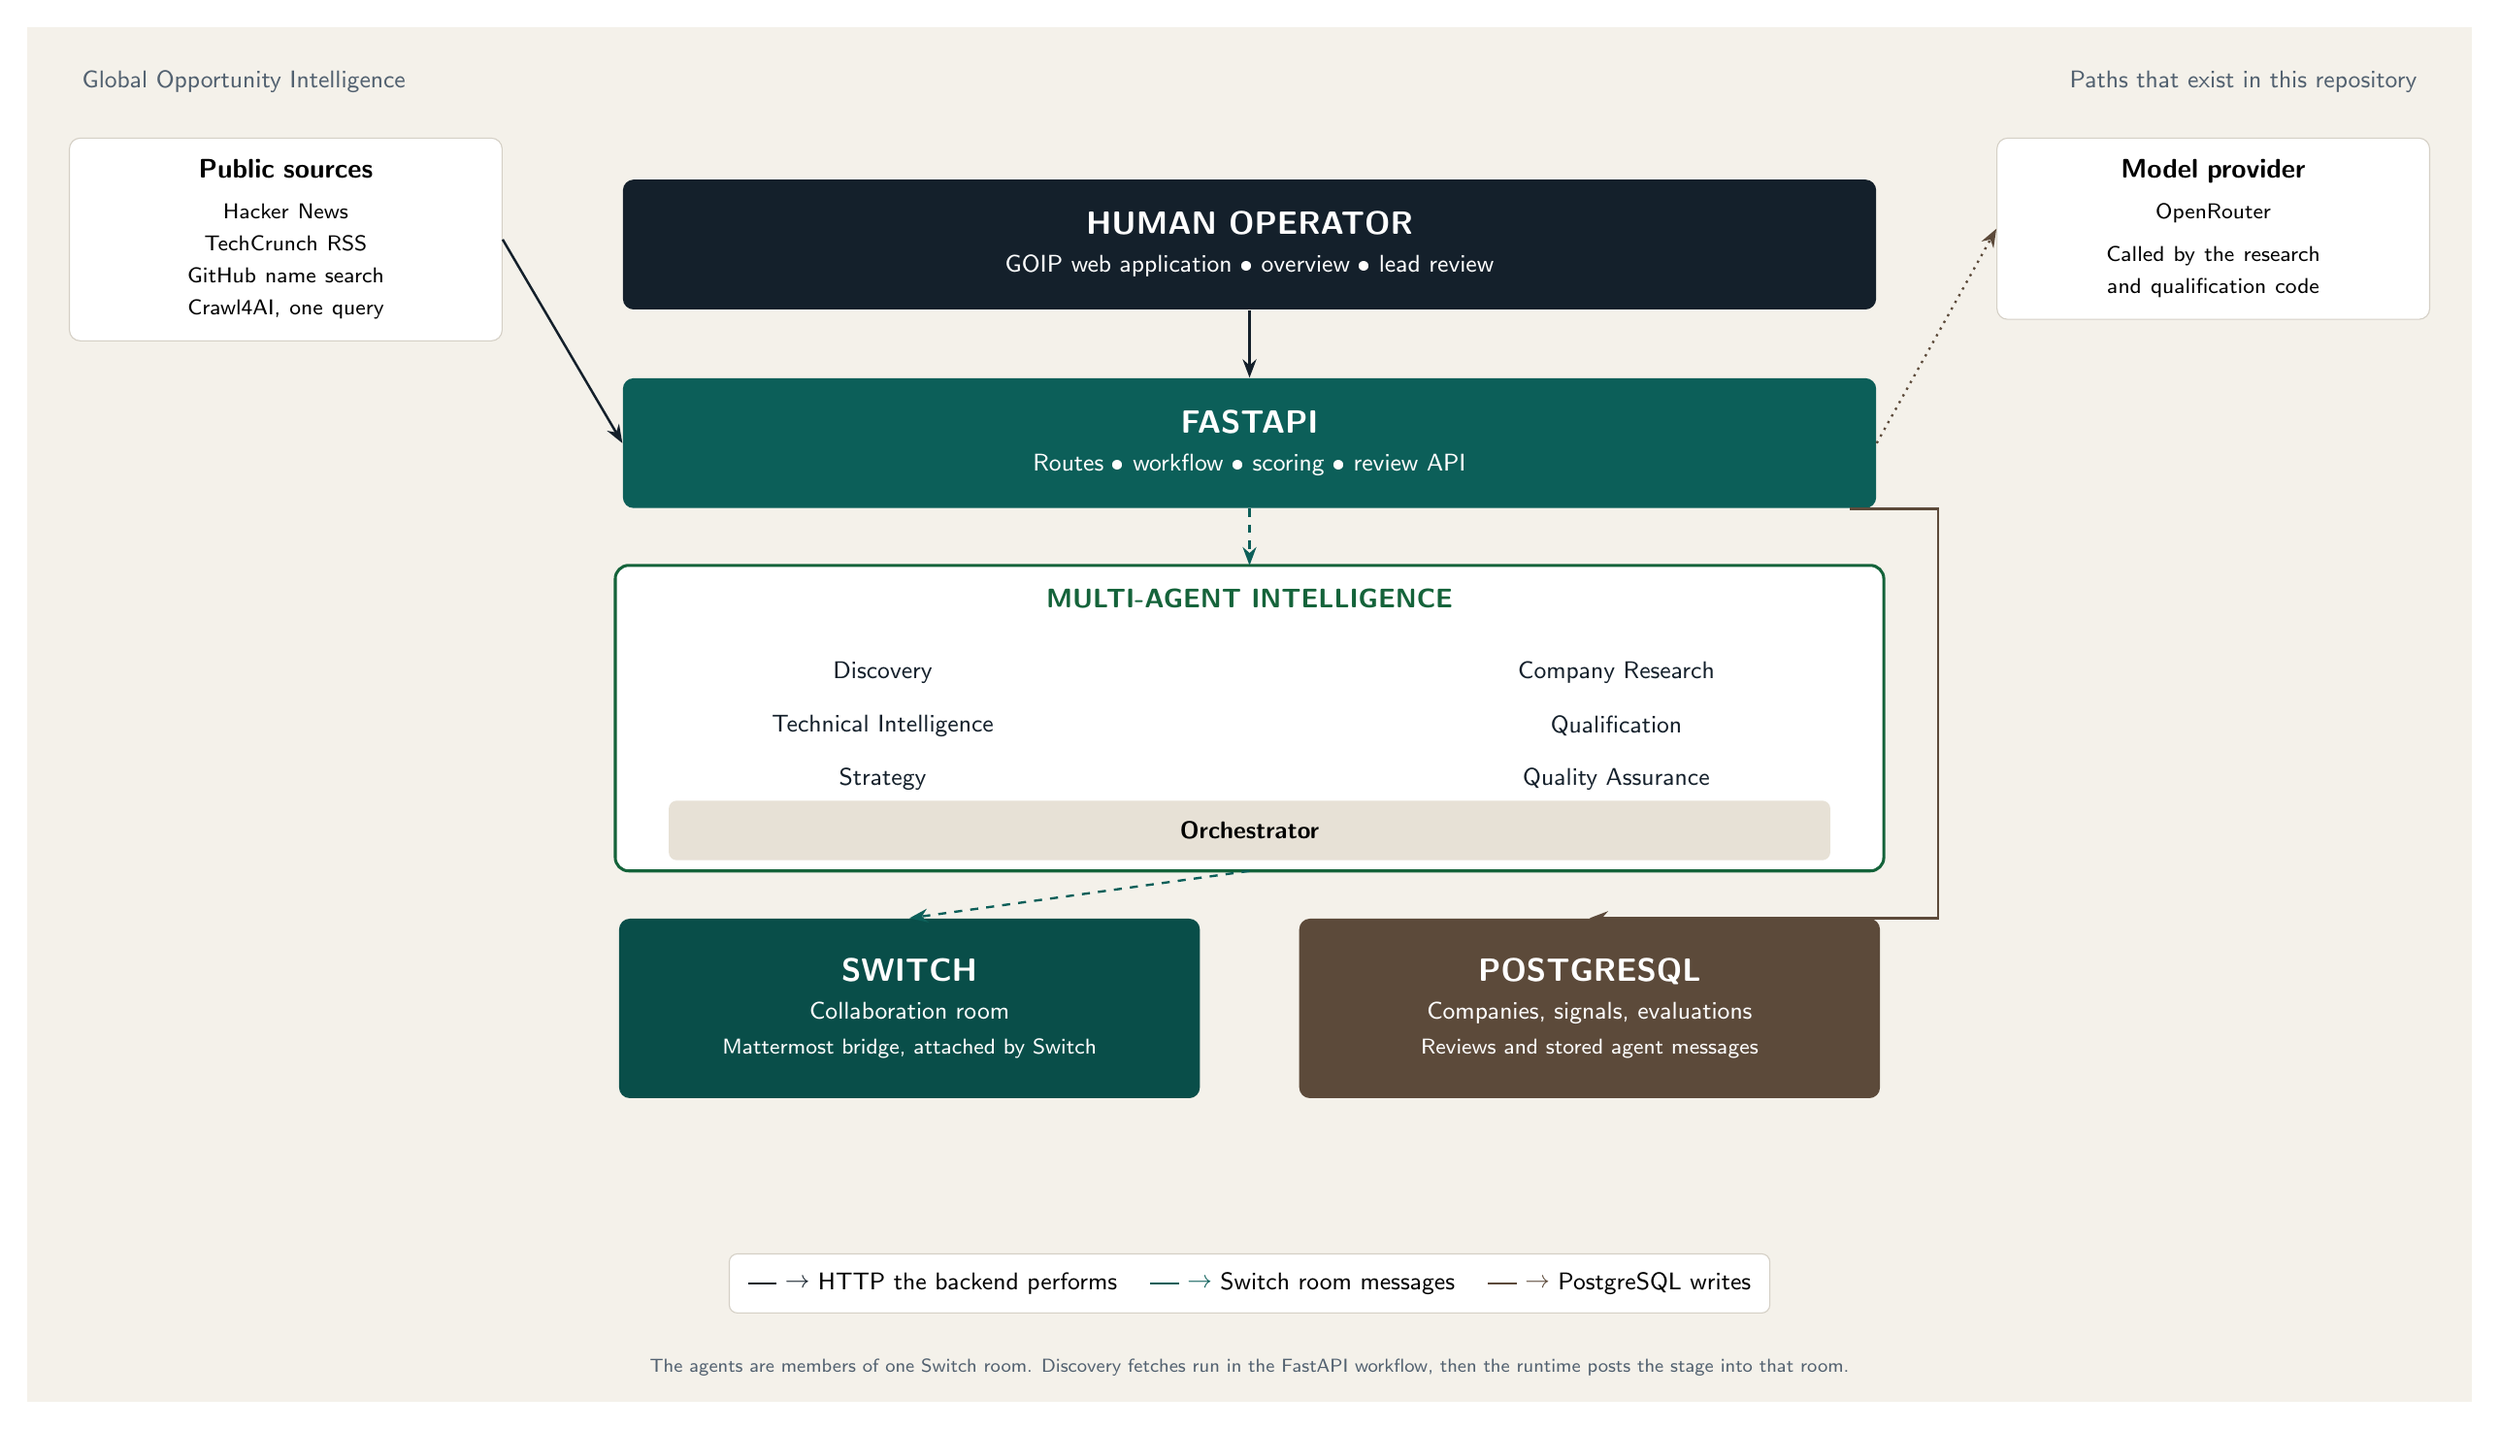
\begin{tikzpicture}[
  x=1cm,y=1cm,
  font=\sffamily,
  >={Stealth[length=2.4mm]},
  flow/.style={->, line width=0.9pt, draw=ink},
  msg/.style={->, line width=0.85pt, draw=teal, dashed},
  model/.style={->, line width=0.85pt, draw=data, dotted},
  store/.style={->, line width=0.9pt, draw=data}
]

\fill[paper] (0,0) rectangle (32,18);

\node[anchor=north west, text=muted, font=\sffamily\small] at (0.6,17.55)
  {Global Opportunity Intelligence};
\node[anchor=north east, text=muted, font=\sffamily\small] at (31.4,17.55)
  {Paths that exist in this repository};

% Side: sources
\node[draw=line, fill=white, rounded corners=4pt, align=center,
      text width=5.1cm, inner sep=8pt, anchor=north west] (sources) at (0.55,16.55) {%
  \textbf{Public sources}\\[3pt]
  {\footnotesize Hacker News}\\
  {\footnotesize TechCrunch RSS}\\
  {\footnotesize GitHub name search}\\
  {\footnotesize Crawl4AI, one query}};

% Side: model
\node[draw=line, fill=white, rounded corners=4pt, align=center,
      text width=5.1cm, inner sep=8pt, anchor=north east] (modelbox) at (31.45,16.55) {%
  \textbf{Model provider}\\[3pt]
  {\footnotesize OpenRouter}\\[4pt]
  {\footnotesize Called by the research}\\
  {\footnotesize and qualification code}};

% Layer 1
\node[fill=ink, text=white, rounded corners=4pt, align=center,
      minimum width=16.4cm, minimum height=1.7cm] (human) at (16,15.15)
  {\textbf{\large HUMAN OPERATOR}\\[2pt]{\small GOIP web application \textbullet\ overview \textbullet\ lead review}};

% Layer 2
\node[fill=teal, text=white, rounded corners=4pt, align=center,
      minimum width=16.4cm, minimum height=1.7cm] (api) at (16,12.55)
  {\textbf{\large FASTAPI}\\[2pt]{\small Routes \textbullet\ workflow \textbullet\ scoring \textbullet\ review API}};

% Layer 3
\draw[agentgreen, line width=1.1pt, rounded corners=5pt, fill=white]
  (7.7,6.95) rectangle (24.3,10.95);
\node[text=agentgreen, font=\sffamily\bfseries] at (16,10.52) {MULTI-AGENT INTELLIGENCE};
\node[text=ink, font=\sffamily\small] at (11.2,9.55) {Discovery};
\node[text=ink, font=\sffamily\small] at (20.8,9.55) {Company Research};
\node[text=ink, font=\sffamily\small] at (11.2,8.85) {Technical Intelligence};
\node[text=ink, font=\sffamily\small] at (20.8,8.85) {Qualification};
\node[text=ink, font=\sffamily\small] at (11.2,8.15) {Strategy};
\node[text=ink, font=\sffamily\small] at (20.8,8.15) {Quality Assurance};
\node[fill=sand, rounded corners=3pt, minimum width=15.2cm, minimum height=0.78cm,
      font=\sffamily\bfseries\small] at (16,7.48) {Orchestrator};

% Layer 4 and 5
\node[fill=tealdeep, text=white, rounded corners=4pt, align=center,
      minimum width=7.6cm, minimum height=2.35cm] (switch) at (11.55,5.15)
  {\textbf{\large SWITCH}\\[2pt]{\small Collaboration room}\\[1pt]{\footnotesize Mattermost bridge, attached by Switch}};
\node[fill=data, text=white, rounded corners=4pt, align=center,
      minimum width=7.6cm, minimum height=2.35cm] (db) at (20.45,5.15)
  {\textbf{\large POSTGRESQL}\\[2pt]{\small Companies, signals, evaluations}\\[1pt]{\footnotesize Reviews and stored agent messages}};

% Legend
\node[draw=line, fill=white, rounded corners=3pt, inner sep=7pt, font=\sffamily\small] at (16,1.55) {%
  \textcolor{ink}{\rule[0.45ex]{1.15em}{0.7pt}}~\raisebox{0.15ex}{\textcolor{ink}{$\rightarrow$}}~HTTP the backend performs
  \quad
  \textcolor{teal}{\rule[0.45ex]{1.15em}{0.7pt}}~\raisebox{0.15ex}{\textcolor{teal}{$\rightarrow$}}~Switch room messages
  \quad
  \textcolor{data}{\rule[0.45ex]{1.15em}{0.7pt}}~\raisebox{0.15ex}{\textcolor{data}{$\rightarrow$}}~PostgreSQL writes};

\node[text=muted, font=\sffamily\scriptsize, align=center] at (16,0.45)
  {The agents are members of one Switch room. Discovery fetches run in the FastAPI workflow, then the runtime posts the stage into that room.};

% Arrows
\draw[flow] (human.south) -- (api.north);
\draw[flow] (sources.east) -- (api.west);
\draw[model] (api.east) -- (modelbox.west);
\draw[msg] (api.south) -- (16,10.95);
\draw[msg] (16,6.95) -- (switch.north);
\draw[store] (api.south east) ++(-0.35,0) -- ++(1.15,0) |- (db.north);

\end{tikzpicture}
\end{document}
